\documentclass{kththesis}

% remove this if you are using XeLaTeX or LuaLaTeX
\usepackage[utf8]{inputenc}

% Use natbib abbreviated bibliography style
\usepackage[square,numbers]{natbib}

\usepackage{amsmath,amsthm,amssymb}
\usepackage{graphicx}
\bibliographystyle{unsrtnat}

%\usepackage{natbib}
%\bibliographystyle{agsm}

\usepackage{lipsum} % This is just to get some nonsense text in this template, can be safely removed

\title{Estimating game level difficulty using Monte Carlo tree search and deep learning}
\alttitle{Uppskattning av spelbanors svårighetsgrad med Monte Carlo tree search och deep learning}
\author{Sami Purmonen}
\email{purmonen@kth.se}
\supervisor{Karl Meinke}
\examiner{Olov Engwall}
\programme{Master in Computer Science}
\school{School of Computer Science and Communication}
\date{\today}


\begin{document}

% Title page
\flyleaf

\begin{abstract}
We explore the usage of Monte Carlo tree search and deep learning in order to estimate game level difficulty. A deep convolutional neural network is trained on large amounts of game play data in order to predict moves from game states. The neural network is then used in a Monte Carlo Tree search algorithm to guide its search. We find that this method improves the estimations.
\end{abstract}

\clearpage

\begin{otherlanguage}{swedish}
  \begin{abstract}
  \end{abstract}
\end{otherlanguage}

\cleardoublepage

\tableofcontents


% This is where the actual contents of the thesis starts
\mainmatter

\chapter{Introduction}
\begin{figure}
\label{fig:difficulty_curve}
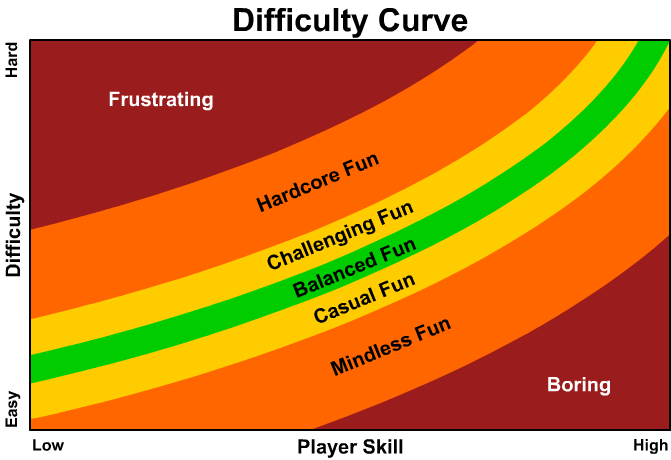
\includegraphics[width=\textwidth]{images/difficulty_curve.png}
\caption{Fun as a function of difficulty and skill}
\end{figure}
Playing games can be fun – but only if the game levels are not too hard nor too easy. Determining how difficult a game level is before releasing it to players is difficult. It is useful for game companies and level designers to have tools for estimating game level difficulty automatically in order to meet the players expectations. Making a game fun is dependent on the game being sufficient difficult with respect to the players skills as demonstrated in Fig. \ref{fig:difficulty_curve}.

We measure game level difficulty as $success/attempts$ for average human players. If we could create a bot that learned the average human players game strategy estimating game level difficulty would be trivial.  We would only need to run the bot on a new level and then have the answer. A game strategy  is defined as a probability distribution $P(A|S)$ over all legal actions $A$ in state $S$.

Erik Poromaa showed that Monte Carlo tree search can perform  accurate estimations of game  level difficulty in Candy Crush as a master thesis student at King  in 2016.

During the same year Google DeepMind showed that Monte Carlo tree search can be improved by including a playout heuristic based on deep learning when creating AlphaGo, a computer Go program  that managed to beat  Lee Sedol in Go.

In this thesis we further explore the problem of estimating game level difficulty in the context of Candy Crush by extending the Monte Carlo tree search with a playout heuristic based on deep learning trained on large amounts of game play data. The game play data was generated from a MCTS bot using a random playout heuristic. If MCTS can be improved by using a playout heuristic learned from itself this could  would suggest that even stronger MCTS can be obtained by training on data generated from the improved MCTS in an iterative procedure. 

\section{Problem}
Our problem is to investigate  if a playout heuristic based on deep learning can improve Monte Carlo tree search and its estimates of game level difficulty.

\section{Delimitation}
We restrict ourselves to one of King's games, Candy Crush Saga, and training on data from a bot based on Monte Carlo tree search. 

\section{Ethics of Artificial Intelligence}
There are two main concerns of Artificial Intelligence. The threat of super intelligence and the economic impact of automatisation.

\subsection{Super Intelligence}
AI can be  divided into three categories  depending on how powerful it is. Today all AI available is in the category Artificial  Narrow Intelligence (ANI) which means that it is task specific. DeepBlue is better than any human being at chess but that is all it can do. The second category is Artificial General Intelligence (AGI) and  includes AI that is about as capable as a human being, meaning that it is capable to do general things that humans can do. The third category is  Artificial Super Intelligence (ASI) and  consists of AI superior to human beings. Once AGI is invented, it is likely going to be able to recursively improve its software in order to make it more capable and eventually reach ASI. This raises concerns about what will happen when humans are not the most intelligent beings on the planet anymore. If ASI turns evil it may spell the end of the human race.  In this thesis we explore yet another application of ANI which in its current state does not pose an existential threat to humanity. No one knows how  we could get from ANI to AGI and since we do not attempt to  do that we do not think the threat of inventing super intelligence is  an ethical concern of this thesis.

\subsection{Economic Impact}
AI capable of replacing human labor  at cheaper prices will cause unemployment, at least temporarily while redundant workers  find replacement work. Some economists are worried that  workers will find it hard to transition to new occupations as they may not have or be capable of acquiring skills demanded.  This thesis might make  manual testers of games redundant and unemployed. We argue that inventing more efficient ways of performing tasks is a good thing even if it temporarily puts some people at an disadvantage. 

\chapter{Relevant Theory}
In this chapter we provide  theoretical foundation that our work is based on. We will take a deeper look into how neural networks work and how they are trained since it is the most important part of this thesis and where a large part of the work has been focused. 
\section{Game Search}
Creating agents playing games commonly use game search algorithms.  The Minimax algorithm has reached state-of-the-art performance in games such as Chess, Checkers and Othello where good heuristics for evaluating game states are available \cite{alphaGo2016}. In games such as Go where it is hard to come up with heuristics, Monte Carlo tree search has instead been the most successful game search algorithm \cite{goMoveEvaluation2014}. 
\subsection{Monte Carlo Tree Search}

\begin{figure}
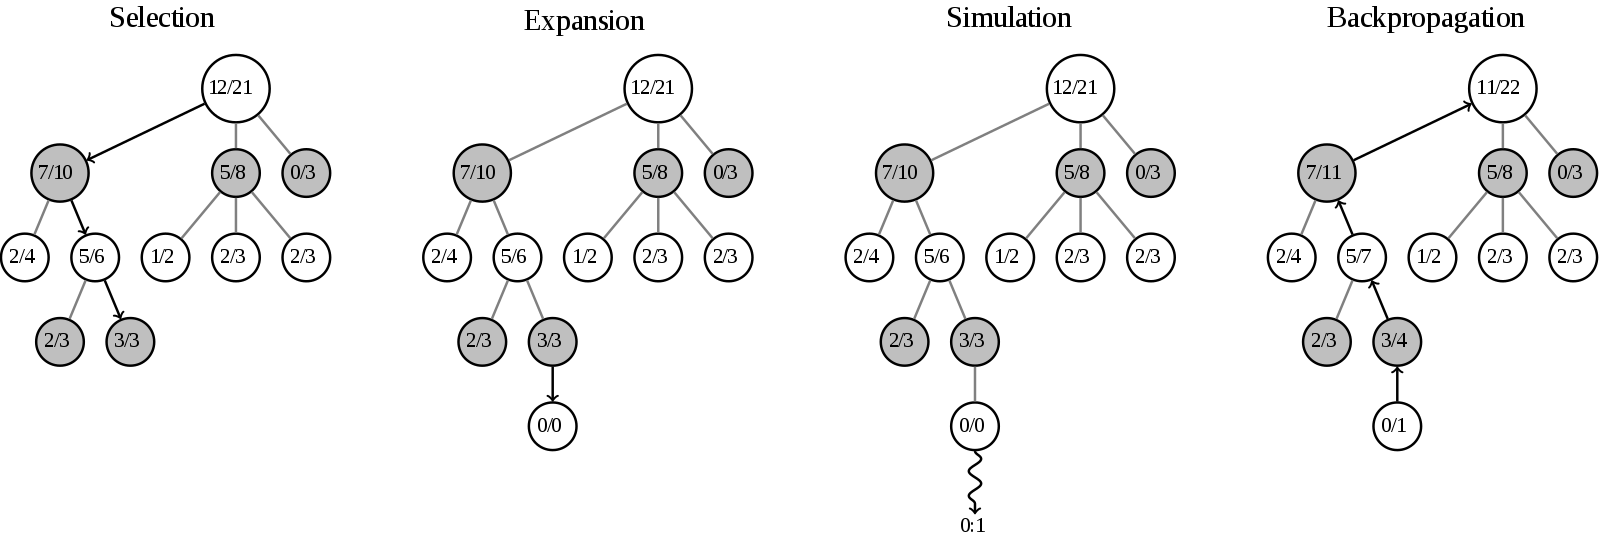
\includegraphics[width=\textwidth]{images/mcst.png}
\label{fig:mcts-steps}
\caption{The steps in a Monte Carlo tree search}
\end{figure}

Monte Carlo tree search  determines the best possible action by simulating game plays from the current state.  During each simulation the search tree is expanded by adding a new node to the search tree. The new node is evaluated by playouts, that is playing to the end, and then determining a score. The scores of the traversed ancestor nodes are updated accordingly. Doing this many times converges to minimax \cite{browne2012survey}.

\section{Machine Learning}
Machine learning  encompasses algorithms that learns by experience. In the most common form, supervised learning, this means that  it learns a function $F: \mathbb{R}^{N} \rightarrow \mathbb{R}^{M}$ from a training set of examples of such mappings and then its prediction on unseen data becomes better, that is it is generalizing. There is also unsupervised learning where the algorithm receives feedback from performing actions and adjusts it is behavior in order to become better at a task. In this paper we are only interested in supervised learning. There are many popular algorithms for supervised learning such as support vector machines and decision trees  but the  one currently receiving most traction is artificial neural networks. 

\subsection{Classification}
Classification means to assign a class $c \in C$ from a finite set  of classes to an input of features. For example, we could have a classifier that takes as input  the height and weight of person and outputs $c \in \{Male, Female\}$. Given a dataset of persons weight and height  labeled with female or male  a  learning algorithm could generate a classifier that predicts the gender of persons.  The usage of course, is to be able to use the classifier on unseen data so the goal during training is to train a classifier that generalizes to unseen data.

\newcommand{\argmax}[1]{\underset{#1}{\operatorname{arg}\,\operatorname{max}}\;}
\subsubsection{Data representation}
\label{sec:machine_learning:data_representation}
The input to a classifier is a vector $X \in \mathbb{R}^{n}$ where $n$ is the  number of features.
The output of the classifier is a vector $Y \in \mathbb{R}^{c}$ where $c$ is the number of classes and $Y_{i}$ is the score of class $i$. The predicted class is $\argmax{i}Y_{i}$. $Y$ can be normalized so that $\sum_{i}Y_{i}=1$ making it a conditional probability distribution over the given classes $P(i|X)=Y_i$ using the softmax function as shown in equation \ref{eq:softmax}. There  is a natural pairing between the cross entropy cost function and softmax activation function \cite{dunne1997pairing}.
\begin{equation}
\label{eq:softmax}
Y_i=\frac{e^{Y_i}}{\sum_j{e^{Y_j}}}
\end{equation}

This is the way we will think of classification in this thesis – a way to generate a probability distribution over all possible classes from an input vector.



\subsection{Artificial Neural Network}
\begin{figure}
\centering
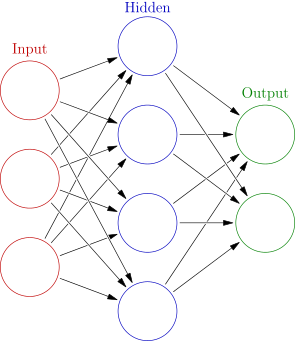
\includegraphics[width=0.5\textwidth]{images/ann.png}
\caption{Fully-connected artificial neural network with one hidden layer}
\label{fig:ann}
\end{figure}

A neural network is a supervised learning algorithm. We will discuss how it is used for the task of classification. A neural network consists of layers  of neurons connected to each other with weights. We will discuss feed-forward neural networks where neurons at layer $i+1$ are only connected to neurons at layer $i$, as shown in Fig. \ref{fig:ann}. Neural networks where neurons have backward connections are called recurrent neural networks and are useful in speech recognition where time is important.  Artificial neurons are loosely modeled after biological  neurons inside the brain. However, we will  think of them as mathematical units since the connection to biology does not ease the understanding of  how they work unless one has a background in biology.

\subsubsection{From input to output}
A neural network used for classification takes an input vector $X \in \mathbb{R}_{n}$ and outputs a vector $Y \in \mathbb{R}_{c}$ representing a probability distribution over the possible classes, as described in \ref{sec:machine_learning:data_representation}. What is different between a neural network and other classifiers is how it does it. That is what we will discuss next. 

\subsubsection{Work of the neuron}
Each neuron  has a weight for each input feature and a bias. It calculates a weighted sum of its inputs which consists of activations from previous layers, as seen in equation \ref{eq:neuron_activation} and applies an activation function. The idea behind the activation function is that the neuron  has a binary output, it either fires or does not. Each neuron detects  patterns  in  input from previous layers and fires when it sees it.  It  also introduces non-linearity in the network which is necessary to be able to approximate non-linear functions.
\begin{equation}
\label{eq:neuron_activation}
A_{j}=g((\sum_{i}W_{ji}X_{i})+b_j)
\end{equation}


A common activation function is the $sigmoid$ as seen in equation \ref{eq:sigmoid}. 

\begin{figure}
\centering
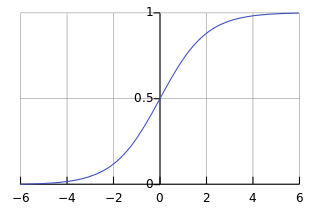
\includegraphics[width=0.5\textwidth]{images/sigmoid.png}
\label{fig:sigmoid}
\caption{Sigmoid function}
\end{figure}

\begin{equation}
\label{eq:sigmoid}
sigmoid(x)=\frac{1}{1+e^{-x}}
\end{equation}
It has been shown that another activation function, the rectified linear unit, is several times faster to train because it is non-saturating \cite{krizhevsky2012imagenet}. It is currently the most popular activation function used  in deep learning \cite{lecun2015deep}.

\begin{figure}
\centering
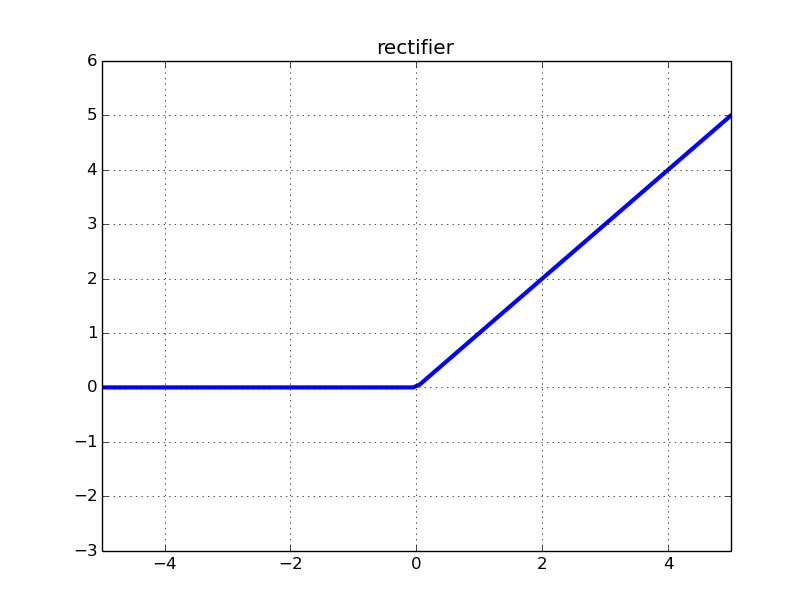
\includegraphics[width=0.5\textwidth]{images/relu.png}
\label{fig:relu}
\caption{ReLU function}
\end{figure}

\begin{equation}
\label{eq:relu}
ReLU(x)=max(x,0)
\end{equation}


\subsubsection{Cost function}
In order to  improve the neural network  there must be an objective measurement of how good or bad the network does. This is captured with a cost function. If the networks output is close to the desired output, the cost is low, otherwise high. A commonly used cost function is mean square error as shown in equation \ref{eq:cost}. 

\begin{equation}
\label{eq:cost}
C =\frac{1}{2}(f(x)-y)^2
\end{equation}

Another commonly used cost function is cross entropy which has significant practical advantages as it finds better local optimums when weights are randomly initialized \cite{golik2013cross, kline2005revisiting}.

\begin{equation}
\label{eq:cross_entropy}
C(p,q) = -\sum_{c}p(c)\log{q(c)}
\end{equation}

\subsubsection{Learning}
The network learns by calculating the cost function and updating its weights in order to minimize the cost function. The learning process is thus an optimization problem.  The cost function is a function of the weights. In order to minimize it gradient descent is used. Gradient descent  calculates the gradient of the cost function with respect to to the weights. It then updates the weights in the opposite direction as to make the cost smaller as seen in \ref{eq:weight_update_derivative}. How big the weight differences are is  decided by the learning rate. In practice stochastic gradient descent is used where only a small subset of the training data is used to calculate an estimate of the cost function which makes the training time faster \cite{michaelnielsen2015}.

\begin{equation}
\label{eq:weight_update_derivative}
w_i= w_i-\lambda\frac{\partial{C}}{\partial{w_i}}
\end{equation}

\subsubsection{Hyper Parameters}
A neural network has many hyper parameters that are not tuned while training. 
\begin{itemize}
\item Learning rate
\item Number of hidden layers
\item Number of hidden nodes
\item Choice of activation function
\item Choice of error measurement
\item Learning rate decay
\item Regularization
\item Initial weights
\end{itemize}
These can be decided by manually testing different combinations. A more rigorous way to choose them is a grid search or random search. In a grid search a finite set of values for each parameter is chosen then all combinations are tried. The one yielding the highest accuracy is selected as the best parameter combination. A random search selects parameters by random which has shown to be more efficient than grid search \cite{bergstra2012random}. Genetic algorithms breeding new combinations  by combining previous successful combinations can also be applied. A novel approach based on reinforcement learning for generating architectures using the validation accuracy  on the validation set as feedback has been demonstrated to be capable of generating architectures  that rivals the best human-invented architectures on the CIFAR-10 dataset \cite{DBLP:journals/corr/ZophL16}.

\subsubsection{Transfer Learning}
Sometimes when a large enough dataset is not available it is possible to use a different dataset and transfer knowledge learned from that, this is called transfer learning \cite{torrey2009transfer}.

\subsection{Convolutional Neural Network}
\begin{figure}
\centering
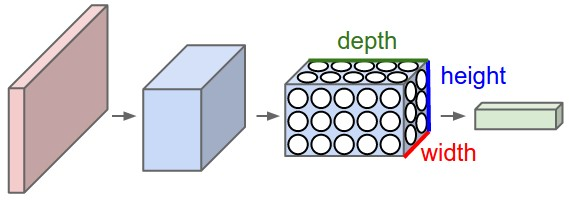
\includegraphics[width=\textwidth]{images/cnn.jpg}
\label{fig:cnn}
\caption{Convolutional neural network}
\end{figure}

Convolutional neural networks have dramatically improved object recognition and is the current state-of-the-art for this task \cite{szegedy2015going}. In a convolutional neural network  each neuron is connected in overlapping tiles giving  the network  locality in a two-dimensional space. This works well for input data that can be treated as images.

\subsubsection{Input}
Instead of treating input data as a 1-dimensional vector it is treated as  3-dimensional data. An  rgb image of size $9\times9$ would have dimensions  $9\times9\times3$ since it has 3 color channels. 

\subsubsection{Patch size}
\begin{figure}
\centering
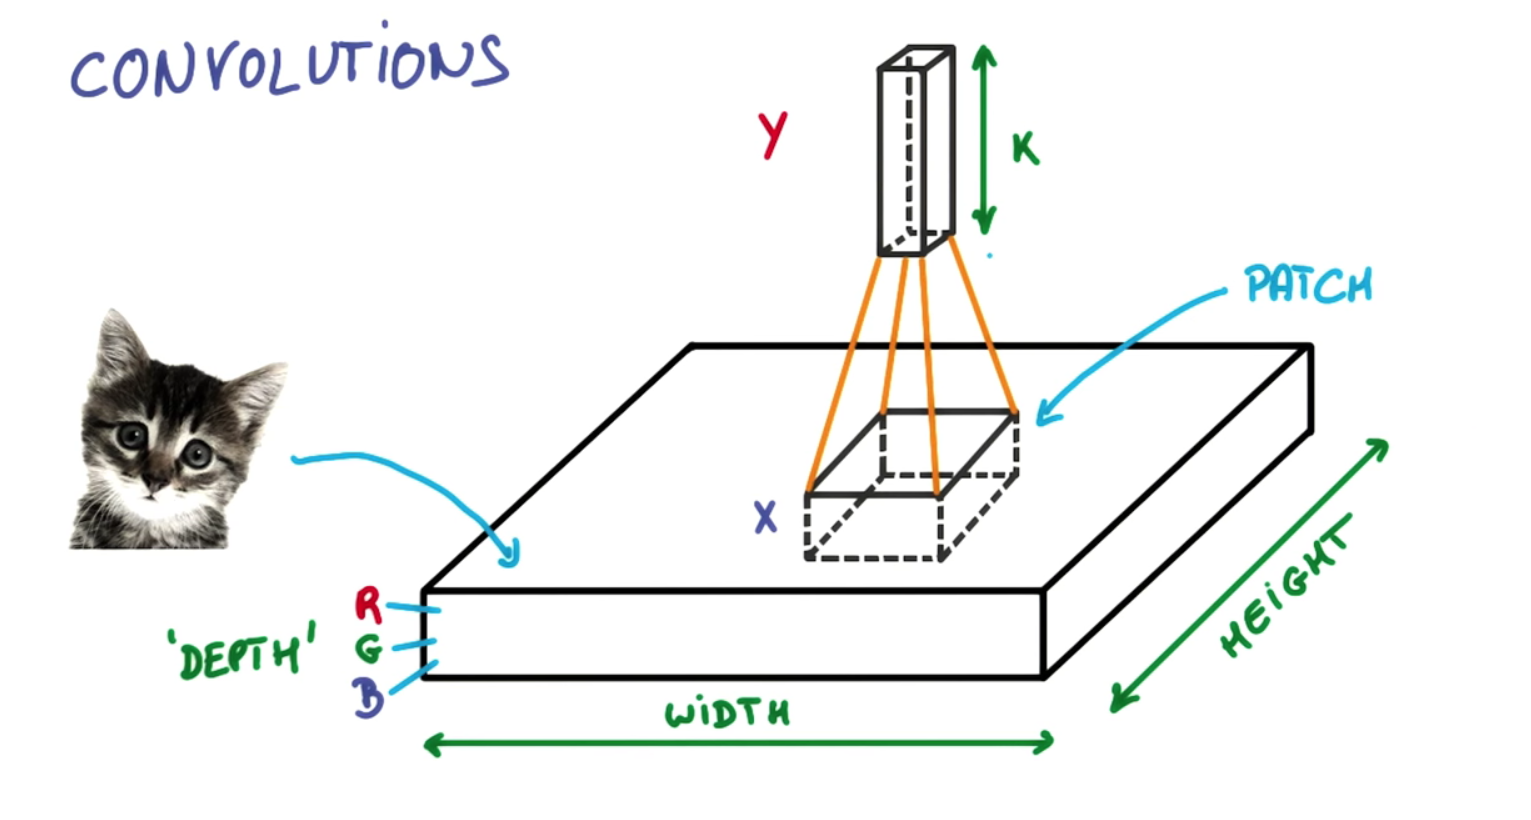
\includegraphics[width=\textwidth]{images/cnn-patch.png}
\label{fig:cnn-patch}
\caption{Patch}
\end{figure}


The patch size determines how large area a neuron covers. A $3\times3$ patch is the most common size and means that each neuron in layer $i+1$ is connected to a  $3\times3$ tile of neurons in layer $i$.

\subsubsection{Stride}
The stride determines the distance between  each neurons inputs.
\subsubsection{Filter}
The number of filters determines how many features can be detected in each layer since the filters share weights.

\subsubsection{Pooling}
Pooling means reducing the dimensions of the input by summarizing its inputs. A $2\times2$ max pooling for example would take an input of $2\times2$ and output $1\times1$ with the highest value found in the input.

\section{Candy Crush}
A few facts.
\begin{itemize}
\item $9\times9$ board size
\item A move consists of swapping two  adjacent tiles 
\item There are 144 possible unique swaps, 72 vertical and 72 horizontal
\item  Only some  swaps are legal such as one creating a match of 3 candies of the same color
\item Goals differ between levels. Sometimes blockers should be cleared, sometimes ingredients must reach the bottom of the screen, sometimes the score must reach a certain level
\item When matching more than 3 candies special candies are created  which are important to do well in the game
\item Solving the game is NP-hard \cite{DBLP:journals/corr/Walsh14}
\item The state space is  huge, the state space on level 13 is approximately $10^{182}$ \cite{poromaa2016}
\end{itemize}

\begin{figure}
\centering
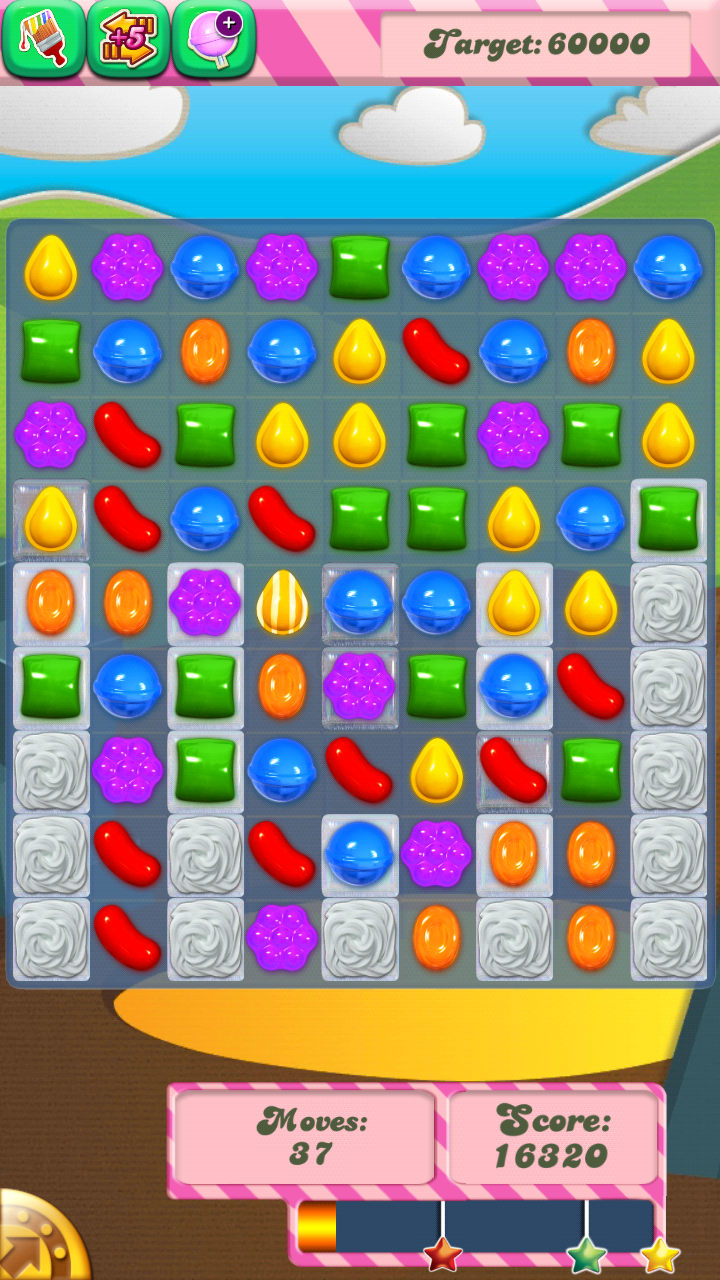
\includegraphics[width=\textwidth]{images/candy_crush.png}
\label{fig:candy_crush}
\caption{Candy Crush}
\end{figure}

\chapter{Related Work}
The primary sources of inspiration comes from  Google Deepminds AlphaGo paper and Erik Poromaas master thesis. Other sources of inspiration comes from image recognition since the problem of predicting moves from game states can be seen as an image recognition problem.  Broader sources of inspiration is anything related to machine learning or AI playing games.


\section{Mastering the game of Go with deep neural networks and tree search}
In "Mastering the game of Go with deep neural networks and tree search" a computer Go program using combinations of supervised learning, reinforcement learning and Monte Carlo tree search is invented. It is the first computer Go program managing to beat professional Go players on a full-sized board. \cite{alphaGo2016}.  

\section{Crushing Candy Crush}
In "Crushing Candy Crush" Erik Poromaa estimates game level difficulty in Candy Crush using Monte Carlo tree search. He finds that this method outperforms previous state-of-the-art methods of manual testing \cite{poromaa2016}.

\section{ImageNet Classification with Deep Convolutional Neural Networks}
In "ImageNet Classification with Deep Convolutional Neural Networks" a large deep convolutional neural network is trained  on millions of high-resolution images  substantially improving previous state-of-the-art in the ImageNet LSVRC-2010 contest \cite{krizhevsky2012imagenet}.

\section{Move Evaluation in Go Using Deep Convolutional Neural Networks}
In "Move Evaluation in Go Using Deep Convolutional Neural Networks" a 12-layer deep convolutional neural network  is trained on a dataset of human professional Go players  to predict moves. It predicts professional moves with 55\% accuracy  and could beat traditional search programs without any search.

\chapter{Method}
In this chapter we give a detailed description of our method. In short it consists of two experiments. 

\section{Simplified Candy Crush}
Because the data is super high-dimensional, and we use a non-deterministic bot for generating data, it might be super hard learning problem.  Also, when the project began no data was available for training. Therefore we decided to:
\begin{enumerate}
\item Build a simplified version of Candy Crush
\item Create a simple deterministic bot playing it
\item Collect data
\item Train a deep neural network 
\item Evaluate the DNN, compare with random accuracy
\item Was it good -> proceed, was it terrible -> reconsider the project
\end{enumerate}
The idea is to use the simplified problem as a playground and give as an early exit point if the problem turns out to be too hard. If we are unable to learn this much simpler learning problem, there is no hope that we will succeed with a much harder one.

\subsection{Simplified Candy Crush}
The simplified version of Candy Crush was implemented in C++ and can be seen in Fig. \ref{fig:candy_small}. It has a slightly smaller game board of $8\times8$ compared to the real game which has $9\times9$. It has 5 different candy colors instead of 6. It has no special candies or blockers and no objectives. The game automatically stops after a 60 seconds and the score increases  proportionally to the number of candies cleared.
\begin{figure}
\centering
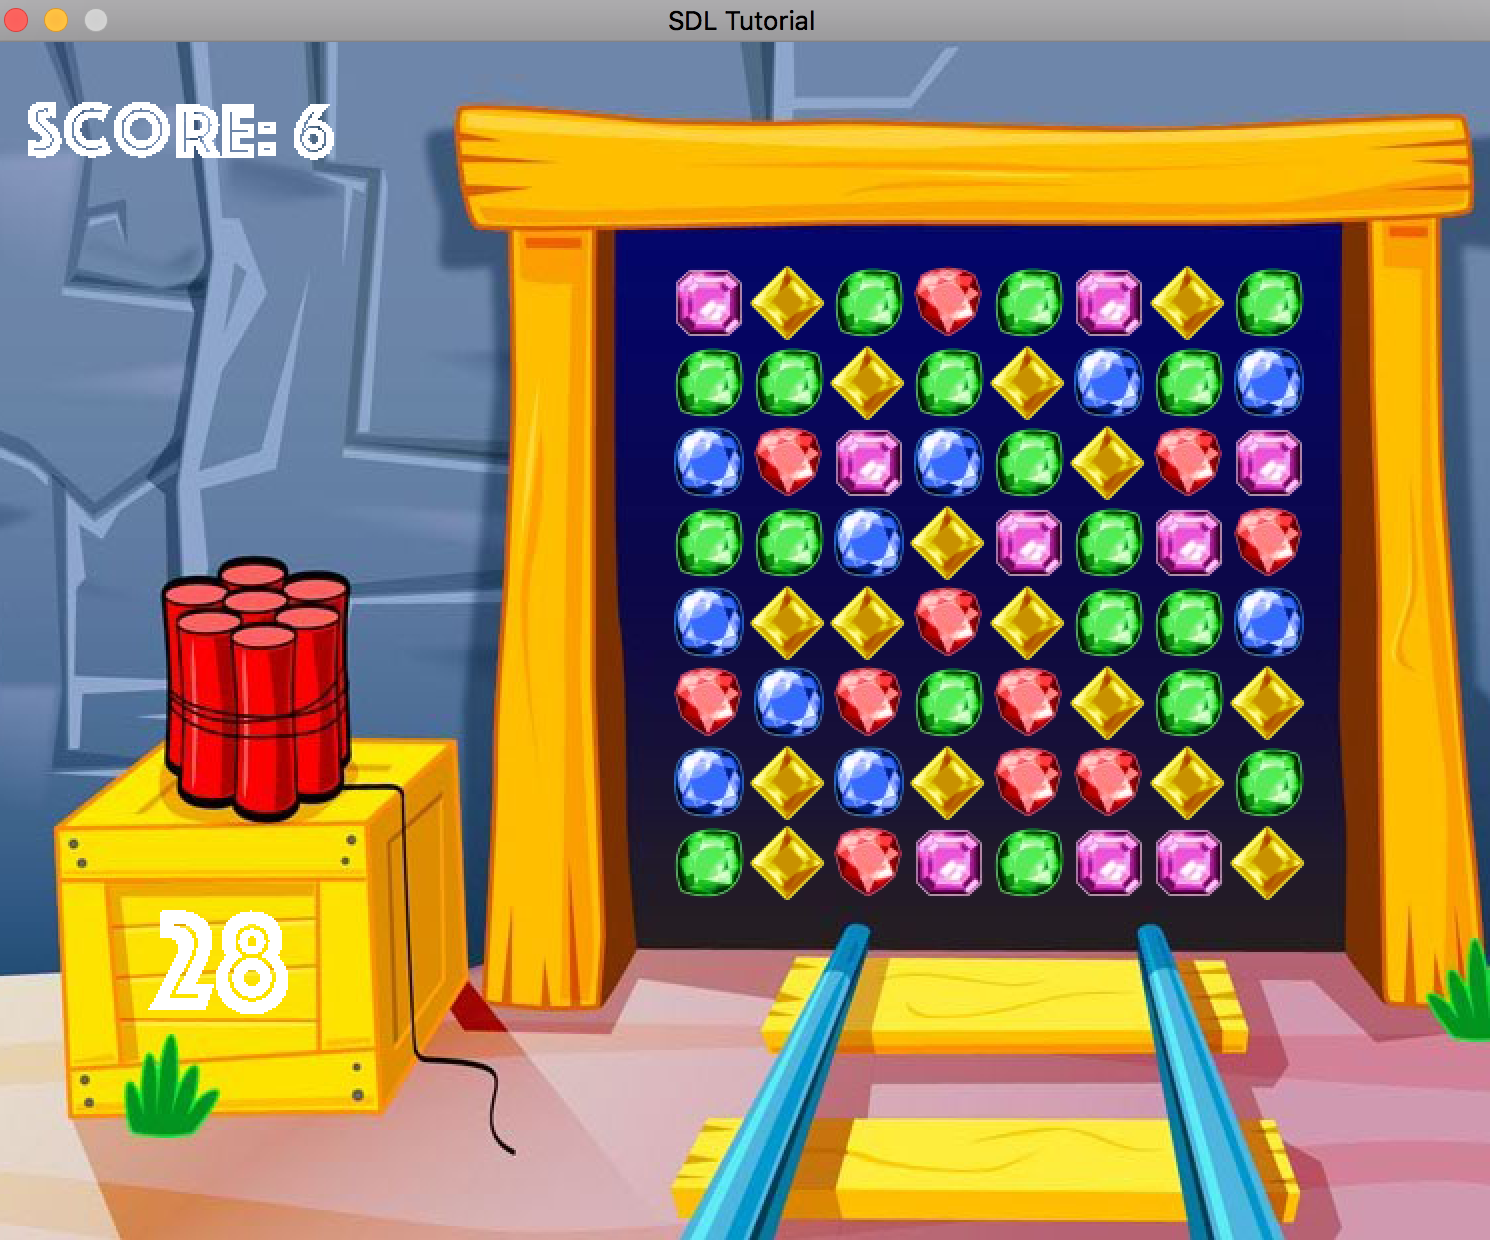
\includegraphics[width=\textwidth]{images/candy_small.png}
\label{fig:candy_small}
\caption{Simplified version of Candy Crush}
\end{figure}

\subsection{Deterministic greedy bot}
The deterministic greedy bot always selects the move which clears the most candies. If there are multiple moves that clears equally many candies, it selects it prefers horizontal swaps to vertical swaps  and north-west positions to south-east positions. This makes the bot completely deterministic and one can from any game board calculate which move it will select.

\subsection{Generating dataset}
We then generated a dataset from a bot playing the game using a deterministic greedy strategy.

It has only two feature planes, one for colors and one for valid moves.

\subsection{Training}
\begin{tabular}{ l | r }
Learning rate & 0.05 \\
Batch size & 128 \\
Patch size & 3 \\
Stride & 1 \\
Filters & 34 \\
Pooling & None \\
Padding & Same \\
Convolutional layers & 3 \\
Fully-connected layers & 1 \\
Hidden nodes & 256 \\
Activation function & ReLU \\
Error measurement & Cross entropy \\
Learning rate decay & 0.96 \\
Regularization & None \\
Initial weights & 0.1 \\
\end{tabular}

\section{Real Candy Crush}
\begin{enumerate}
\item Collect data from Candy Crush (originally intended to use real user data, but after big trouble we aborted)
\item Train a deep neural network using multiple architectures and parameters
\item Evaluate performance using validation accuracy and select the architecture with highest, compare with random accuracy
\item Play the game using DNN, Random, MCTS + DNN, MCTS + Random
\item Evaluate the success rates
\item Make sure results are statistically significant
\end{enumerate}


\chapter{Method}
In this chapter we give a detailed description of our method. In short it consists of the following three steps.
\begin{enumerate}
\item  We  gathered a large dataset of state-action mappings from an MCTS bot playing a diverse set of Candy Crush levels.
\item A deep convolutional neural network was trained on the dataset to predict actions from states.
\item An MCTS bot using the neural network to guide its playouts was used in experiments playing a diverse set of Candy Crush levels and its performance was compared to an MCTS bot using random playouts as well as humans.
\end{enumerate}
   

\section{Deep learning}
The deep  learning classifier is trained to predict moves from game states and is called the move predictor. A move in Candy Crush consists of swapping two adjacent tiles. Only some moves are legal such as ones creating a horizontal or vertical line of 3 or more tiles with the same color.

\subsection{Training Data}
A Candy Crush game board has size 9x9 and  consists of multiple layers of items. A cell can be populated by a normal candy for which there are 6 colors,  blockers or be empty. The training data is divided into feature planes, most of them binary, saying whether a cell has a certain feature.  The 6 colors each have a separate binary feature plane as can be seen in Fig. \ref{fig:game_board} since  the color of a candy has categorical meaning and no numerical relationship. Blockers is a discrete feature plane representing the number of lives left for each blocker. There are in total 36 feature planes. 

\begin{enumerate}
\label{tab:feature_planes}
\item HORIZONTAL MOVES AVAILABLE
\item VERTICAL MOVES AVAILABLE
\item MISSING TILES
\item CANDY COLOR RANDOM
\item CANDY COLOR NONE
\item CANDY BLUE
\item CANDY GREEN
\item CANDY ORANGE
\item CANDY PURPLE
\item CANDY RED
\item CANDY YELLOW
\item NUM CANDY COLORS
\item JELLY
\item BLOCKERS
\item LOCKS
\item BOARD ITEM TYPE NORMAL
\item BOARD ITEM TYPE ROW
\item BOARD ITEM TYPE COLUMN
\item BOARD ITEM TYPE WRAP
\item BOARD ITEM TYPE HOT
\item BOARD ITEM TYPE BOMB
\item BOARD ITEM TYPE SWEDISH FISH
\item BOARD ITEM TYPE INGREDIENT CHERRY
\item BOARD ITEM TYPE INGREDIENT HAZELNUT
\item BOARD ITEM TYPE TIME REFILL
\item BOARD ITEM TYPE PEPPER CANDY
\item BOARD ITEM TYPE LICORICE BLOCKER
\item BOARD ITEM TYPE COCONUT WHEEL
\item BOARD ITEM TYPE JOKER
\item BOARD ITEM TYPE MYSTERY CANDY
\item BOARD ITEM TYPE CHAMELEON CANDY
\item BOARD ITEM TYPE FROG
\item BOARD ITEM TYPE MULOCK KEY
\item BOARD ITEM TYPE UFO
\item NUM BOARD ITEM TYPES
\item NUM MOVES LEFT
\end{enumerate}

\begin{figure}
\centering
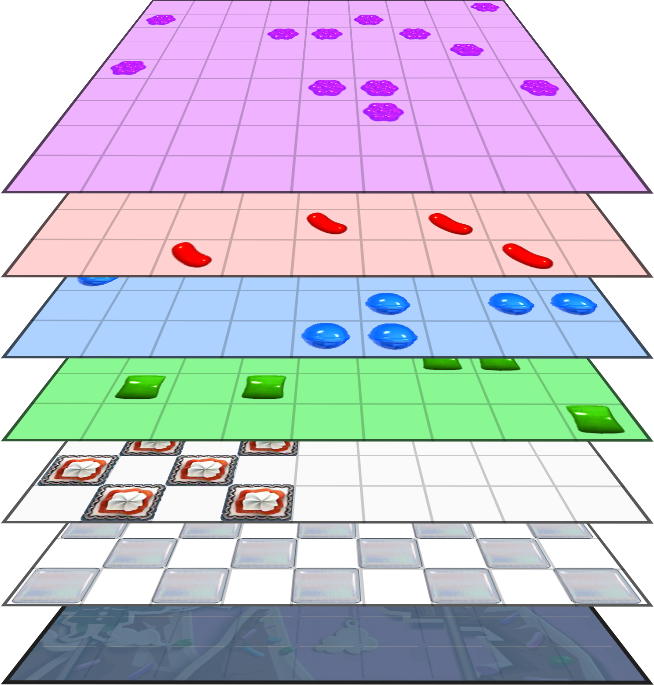
\includegraphics[width=0.8\textwidth]{images/game_board_feature_planes.png}
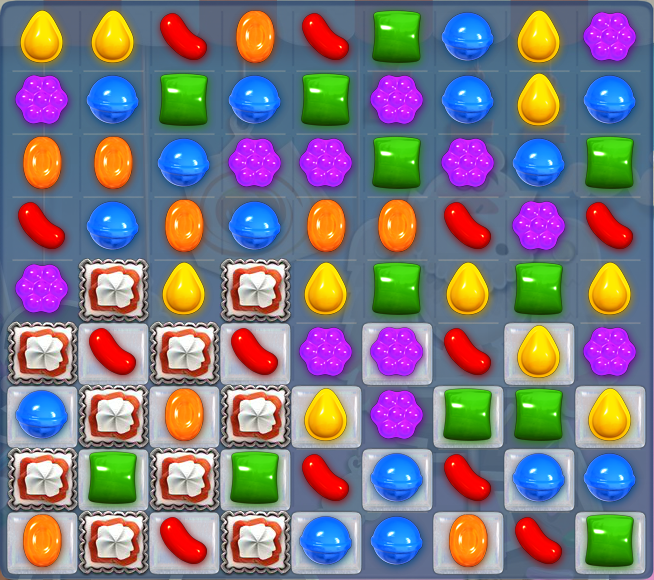
\includegraphics[width=0.8\textwidth]{images/game_board.png}

\label{fig:game_board}
\caption{Example game board and its feature planes}
\end{figure}

There are a few drawbacks with the dataset.  The biggest one is that there is no feature plane for the goal of the level. If the goal is clearing jellies the data does not contain the number of jellies to be cleared or if the goal is to clear ingredients there is no feature plane containing the number ingredients left to be cleared. This will likely make it harder for the network to learn to prioritize the goal when the number of moves left are few rather than creating fancy special candies. Another drawback is that some of the feature planes such as ufo are very rarely, if ever, used. This will likely make it harder for the neural network to learn.
 
We gathered a training dataset of 2 million data points from the MCTS bot playing a diverse set of levels. 50k datapoints was used for validation and the rest was used for training.

\subsection{Network Architecture}
The network architecture was decided by manual experimentation starting with reasonable parameters from prior work. We would have liked to perform a grid search on many combinations of parameters but we deemed that to be too time consuming and computationally expensive to be viable for this work. 

\begin{tabular}{ l | r }
Learning rate & 0.05 \\
Batch size & 128 \\
Patch size & 3 \\
Stride & 1 \\
Filters & 34 \\
Pooling & None \\
Padding & Same \\
Convolutional layers & 3 \\
Fully-connected layers & 1 \\
Hidden nodes & 256 \\
Activation function & ReLU \\
Error measurement & Cross entropy \\
Learning rate decay & 0.96 \\
Regularization & None \\
Initial weights & 0.1 \\
\end{tabular}

\subsection{Software}
We used the deep learning library TensorFlow to implement the neural network. Google created TensorFlow to replace DistBelief which is widely used within Google \cite{abadi2016tensorflow}. TensorFlow is written in C++ with an API available in Python. There are faster deep learning libraries available such as Torch and Theano \cite{bahrampour2015comparative}. TensorFlow was chosen solely because it is hyped and backed by Google and we wanted to explore it.

\subsection{Training}
We used a GPU server from Amazon Web Services for the training.

\subsection{Performance Measures}
The perfomance measured used during training is validation accuracy as seen in equation \ref{eq:validation_accuracy}. 

\begin{equation}
\label{eq:validation_accuracy}
\frac{correct}{total}
\end{equation}

The validation accuracy is not a perfect measurement of game strategy since the selected action in a game state is non-deterministic, meaning that a player in  certain game state multiple times may choose different actions. If a player is in a state with 10 legal actions and the player selects one out of two actions with 50\% probability then the theoretical maximum validation accuracy would be 50\%, but if the network learned the correct probability distribution it would have completely nailed the game strategy. The ideal would be to use a measurement between the distance of the real and predicted probability distributions rather than validation accuracy such as the Kullback–Leibler divergence shown in equation \ref{eq:kullback_leibler_divergence}.

\begin{equation}
\label{eq:kullback_leibler_divergence}
\sum_i P(i)\ln\frac{P(i)}{Q(i)}
\end{equation}

However, since the state space is so large it is very rare that there are multiple training samples from a specific state making it impossible to estimate a probability distribution in the specific state. Validation accuracy is therefore chosen for pragmatic reasons.

Having no other benchmarks this  is compared to the expected accuracy of randomly selecting moves in each game state calculated as $\frac{1}{n}\sum_i^n\frac{1}{S_{i}}$ where $S_{i}$ is the number of moves available in state $i$.


\section{Monte Carlo Tree Search}
\subsection{Implementation}
The Monte Carlo tree search algorithm used was provided by King. It is written in C++ on top of the Candy source code. The implementation has a few novelties. Instead of only using win or loss as the signal a  continuous signal is used based on partial goals such as the number of jellies cleared and/or the score. 

\subsection{Generating training data}
We added logging of all $(state, action)$ pairs  during game play in a CSV-format directly usable for training a neural network in TensorFlow.

\subsection{Using the neural network}
The neural network was used through an HTTP server written in Python because we deemed it to cumbersome to use the at the time immature TensorFlow C++ API as it required us to use Bazel, a build system provided from Google, which interferes with the build system used for Candy. Having the HTTP server on another physical machine caused significant overhead increasing the runtime. This did not matter much as we only ran the experiments a few times but in the future we would probably want to use the neural network natively in C++.

The neural network was used during playouts where the highest probable move was selected.



\section{Experiments}
\subsection{Simplified Candy Crush}
Considering how diverse Candy Crush levels and objectives can be which is demonstrated by the large number of feature planes required to fully describe the game as well as the many and possibly advanced strategies that the user can  have learning  can be really difficult. We decided to start with implementing a simplified version of Candy Crush in C++. It has a slightly smaller game board of $8\times8$ compared to the real game which has $9\times9$. It has 5 different candy colors instead of 6. It has no special candies or blockers and no objectives. We then generated a dataset from a bot playing the game using a deterministic greedy strategy. It has only two feature planes, one for colors and one for valid moves. If we are unable to learn a simple deterministic strategy on this simplified version of the game there is no hope in learning more advanced strategies in the real game. 

\begin{figure}
\centering
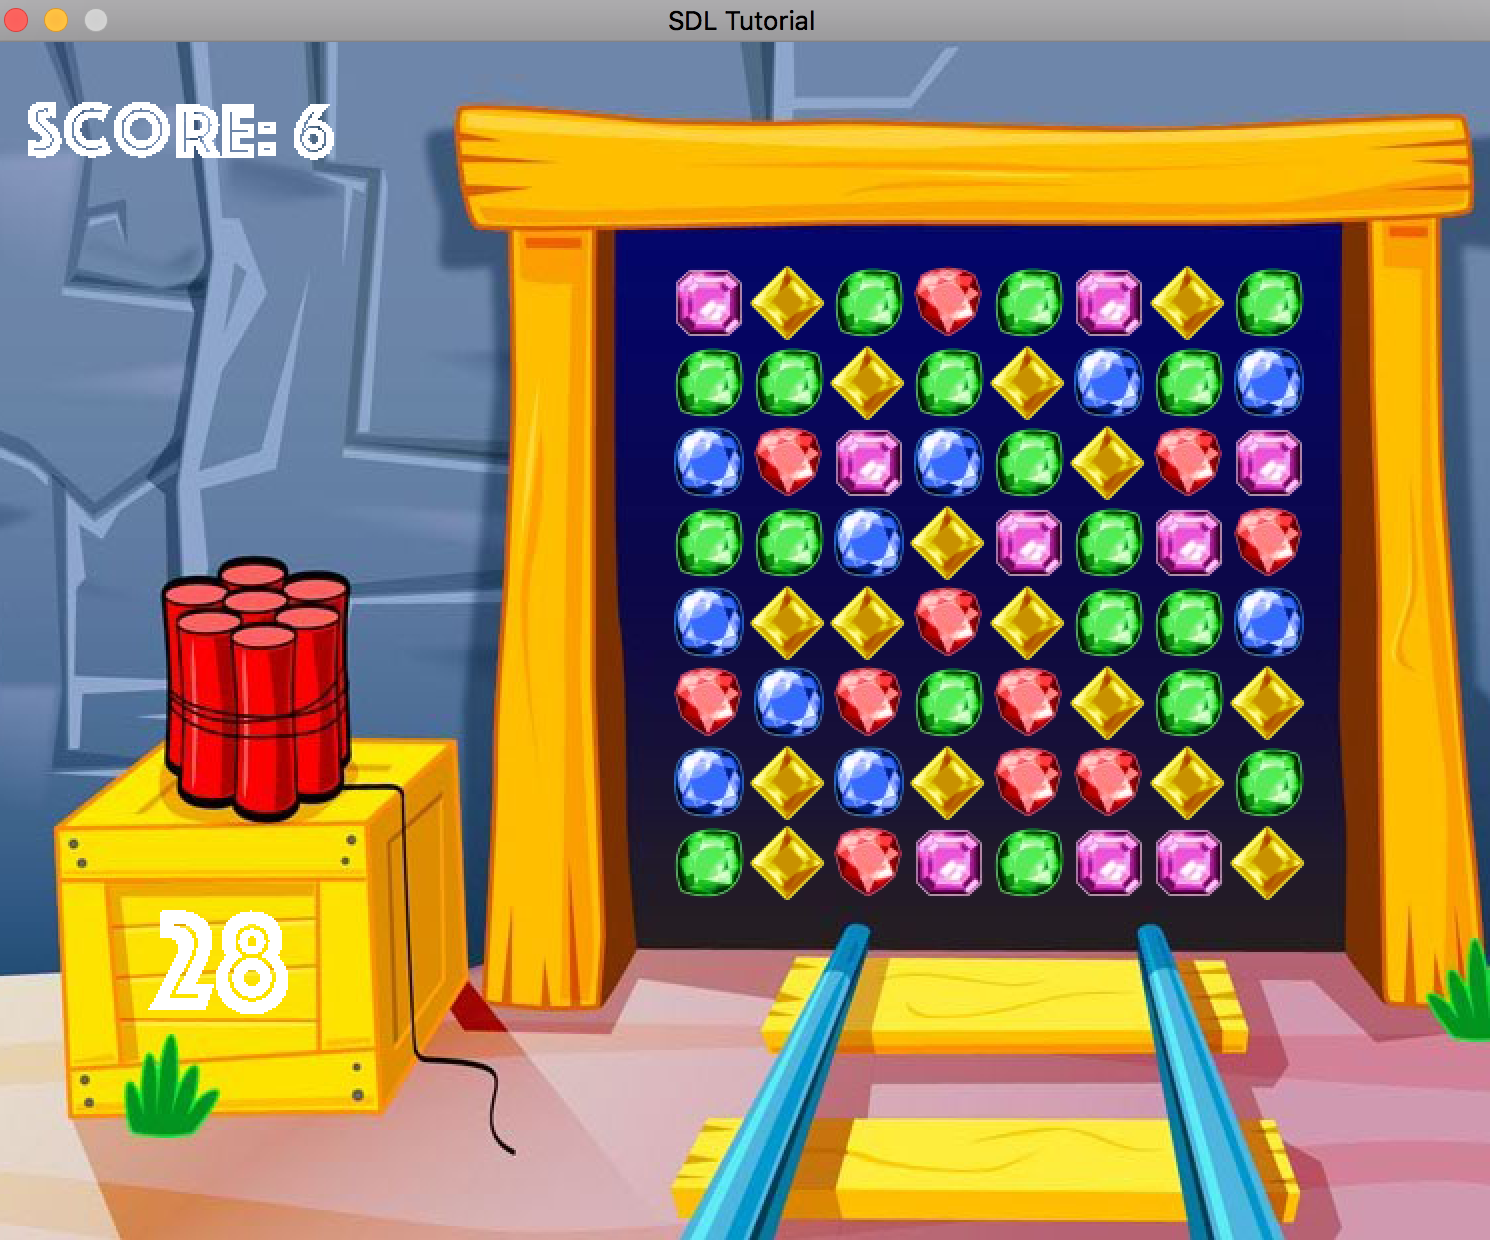
\includegraphics[width=\textwidth]{images/candy_small.png}
\label{fig:candy_small}
\caption{Simplified version of Candy Crush}
\end{figure}

\subsection{Deep learning with MCTS}
We trained a neural network on data generated by an MCTS bot on the real Candy Crush. We created a new MCTS bot using deep learning for playouts and tested it on a diverse  set of levels and compared the results with the previous MCTS bot in order to answer our research question. We also evaluated the results compared to players.
\chapter{Results}

\section{Greedy strategy on simplified version of Candy Crush}

\begin{figure}
\centering
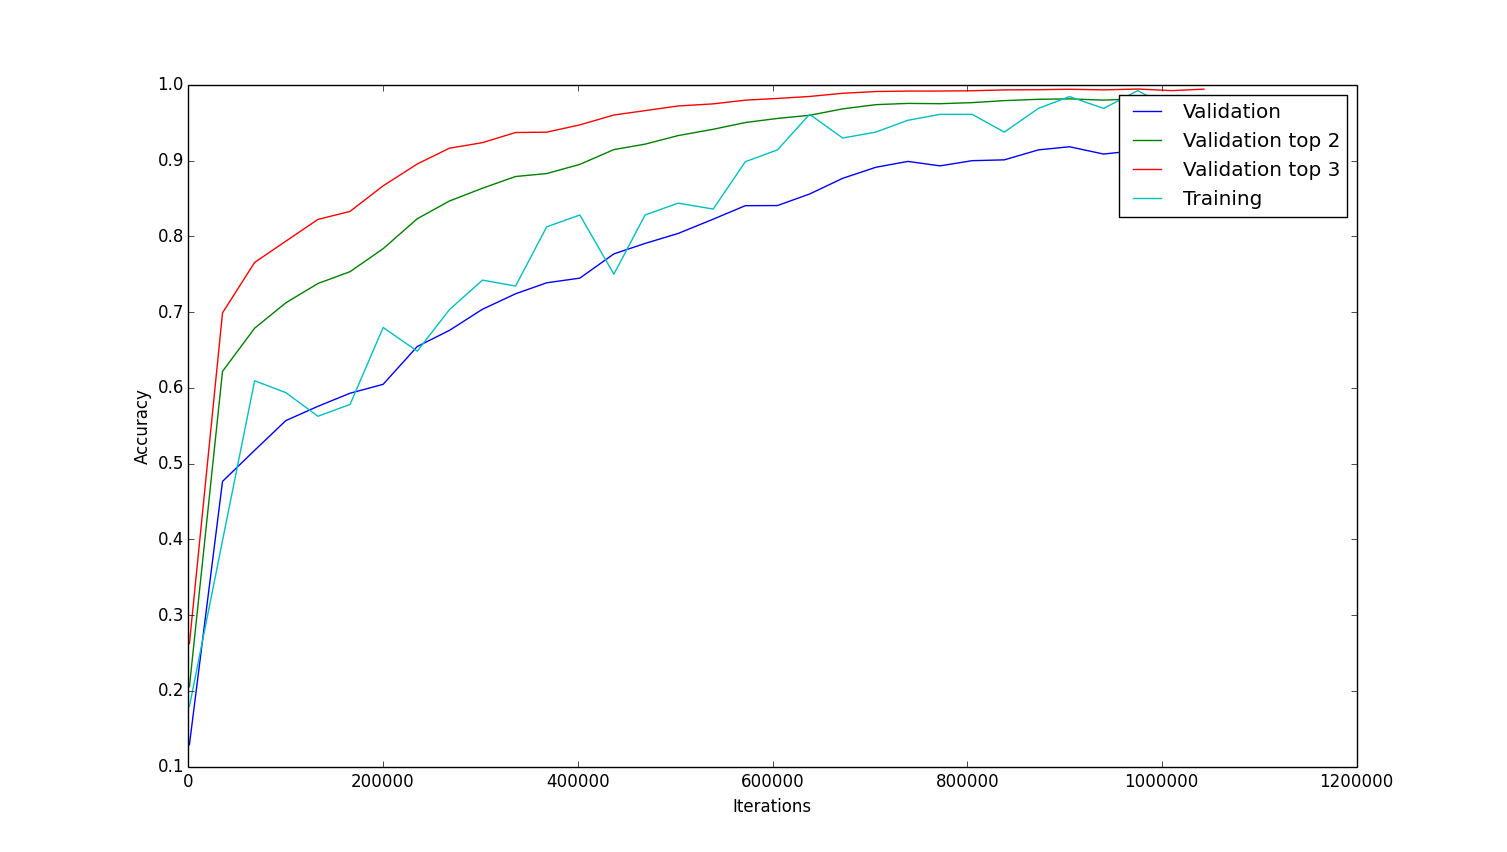
\includegraphics[width=\textwidth]{images/candy_small_validation.png}
\label{fig:candy_small_validation_accuracy}
\caption{Validation accuracy on simplified version of Candy Crush}
\end{figure}


\begin{table}
\caption{Simple data}
\centering
\begin{tabular}{ l | r }
\hline
Training size & 450 176\\
Validation size & 26 000\\
Average number of moves per state & 23.2 \\
Random accuracy & 4.9\% \\
Validation accuracy & 92.2\% \\
Validation top-2 accuracy & 98.3\% \\
Validation top-3 accuracy & 99.4\% \\
Training accuracy & 98.9\% \\
Iterations & 18k \\
Duration & 69h \\
\hline
\end{tabular}
\end{table}

\begin{table}
\caption{Real data}
\centering
\begin{tabular}{ l | r }
\hline
Training size & 1 594 714\\
Validation size & 50 000\\
Average number of moves per state & 13.4 \\
Random accuracy & 16.7\% \\
Validation accuracy & 28.3\% \\
Validation top-2 accuracy & 44.4\% \\
Validation top-3 accuracy & 57.3\% \\
Training accuracy & 30.4\% \\
Iterations & 1 000 000 \\
Duration & 7 days \\
\hline
\end{tabular}
\end{table}


\section{Deep learning training on MCTS data in Candy Crush}

\begin{figure}
\centering
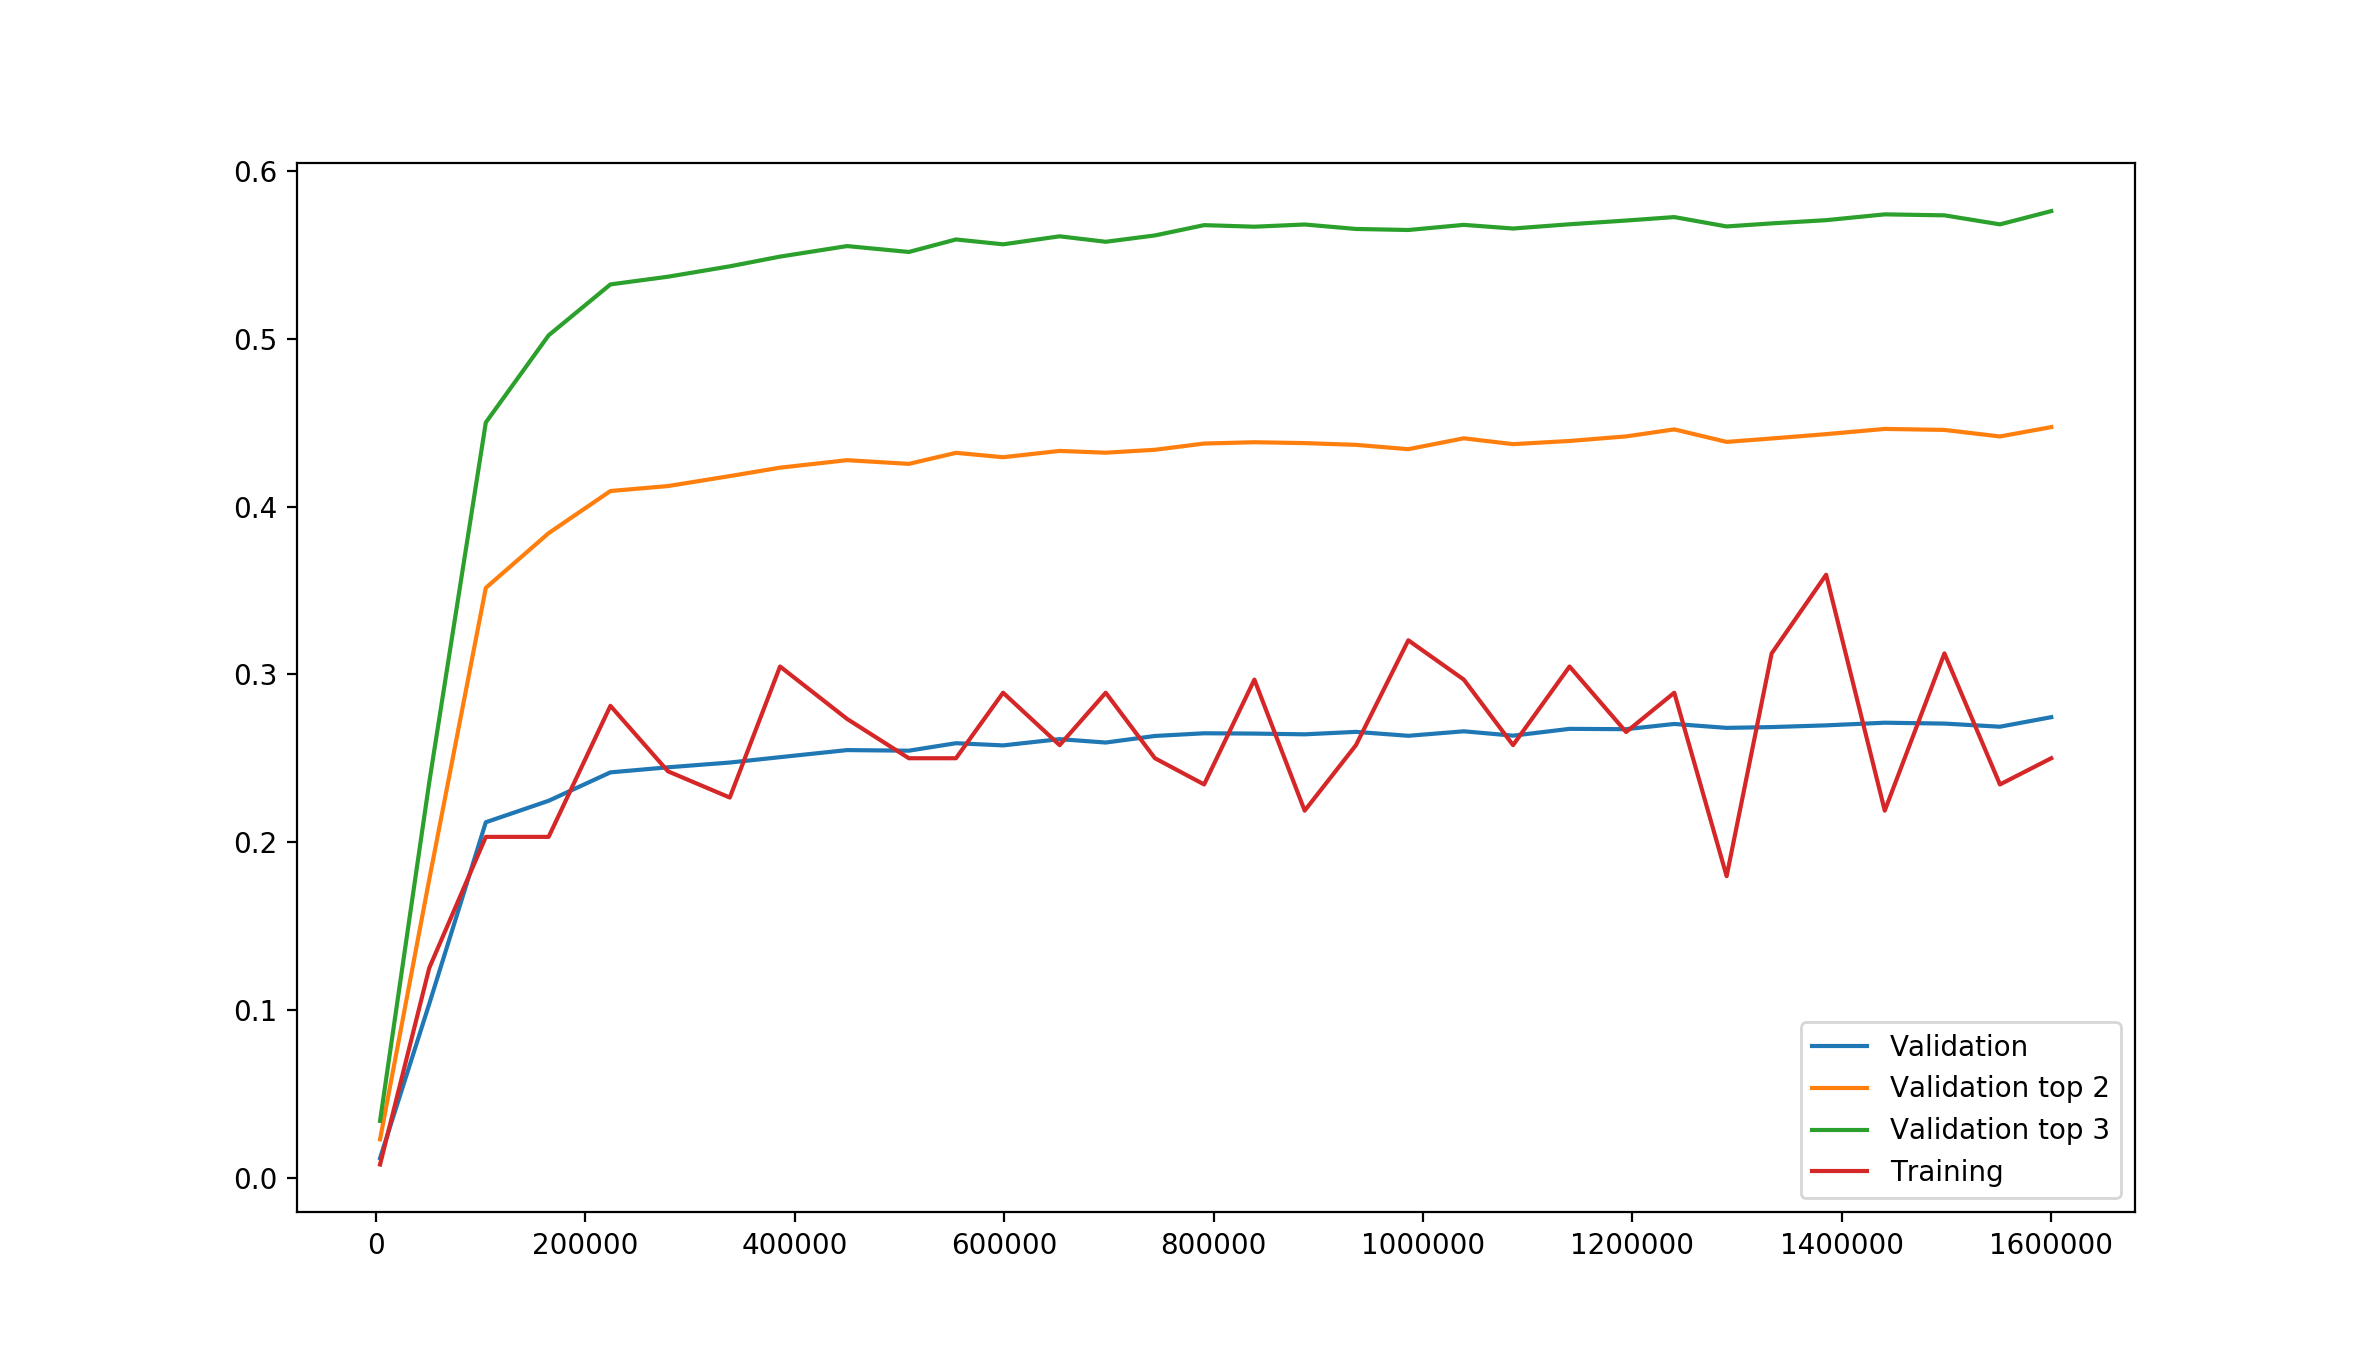
\includegraphics[width=\textwidth]{images/candy_real_training.png}
\label{fig:candy_real_validation_accuracy}
\caption{Validation accuracy on Candy Crush}
\end{figure}

\section{Monte Carlo tree search with deep learning}

\begin{figure}
\centering
w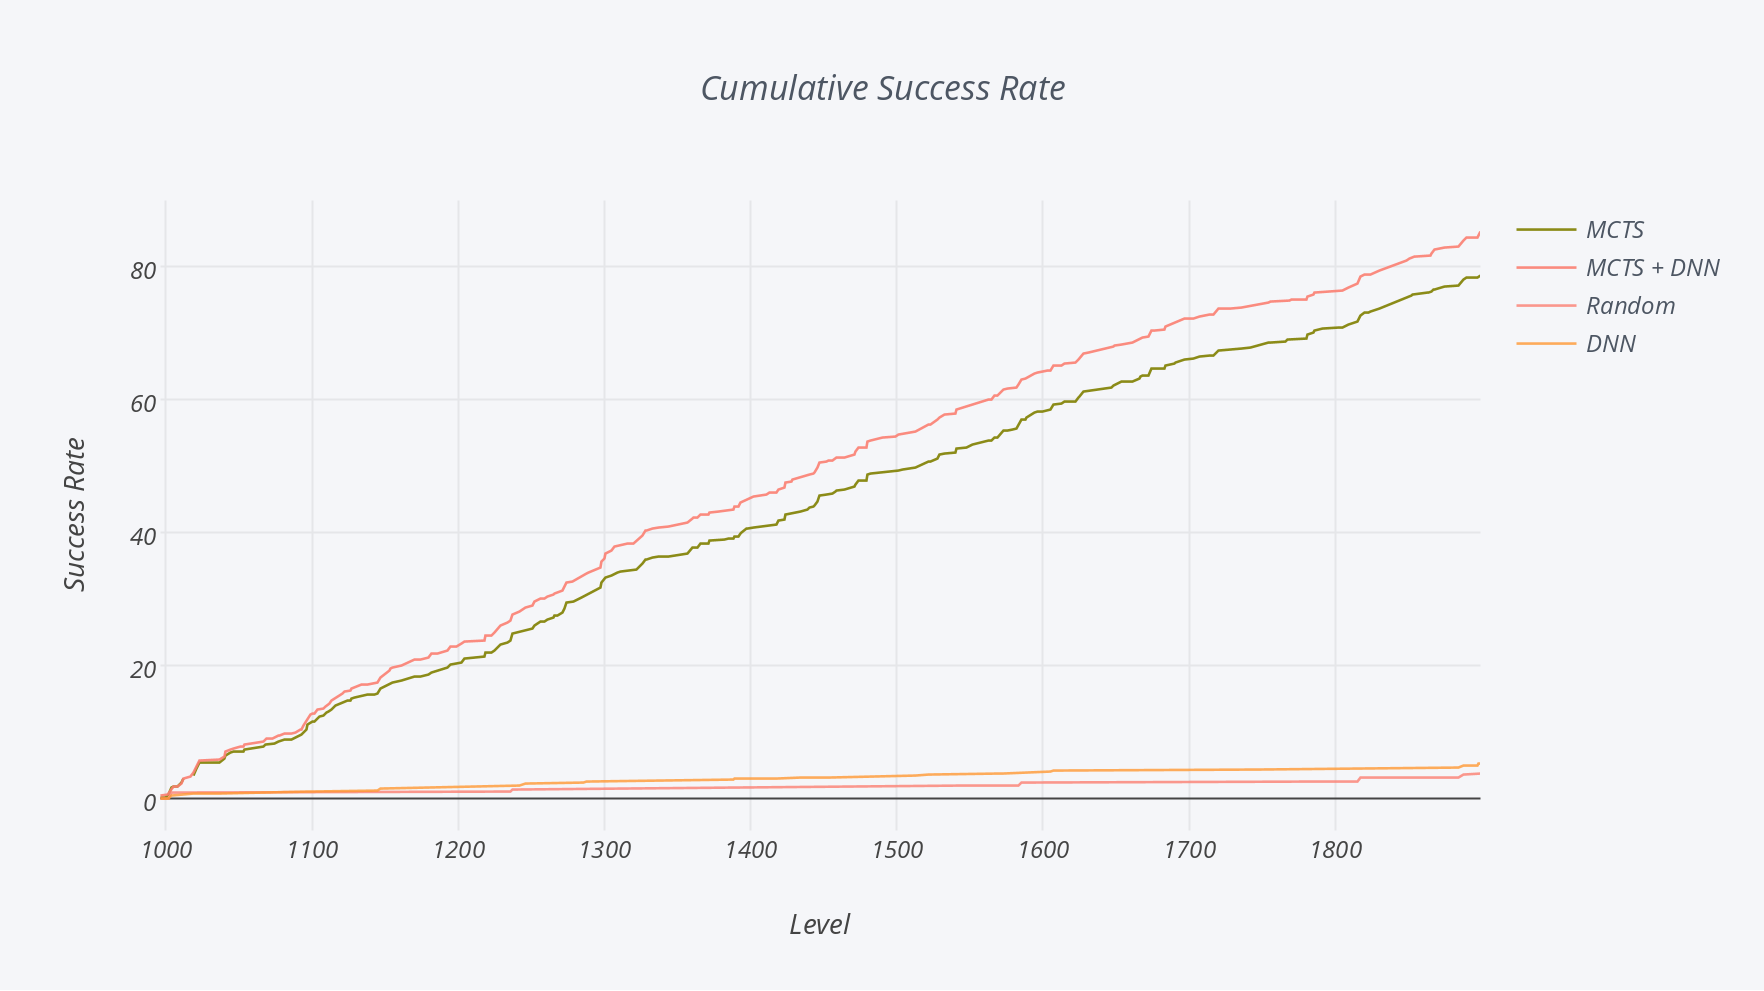
\includegraphics[width=\textwidth]{images/cumulative_sr.png}
\label{fig:cumulative_sr}
\caption{Cumulative success rate for each method}
\end{figure}

\begin{figure}
\centering
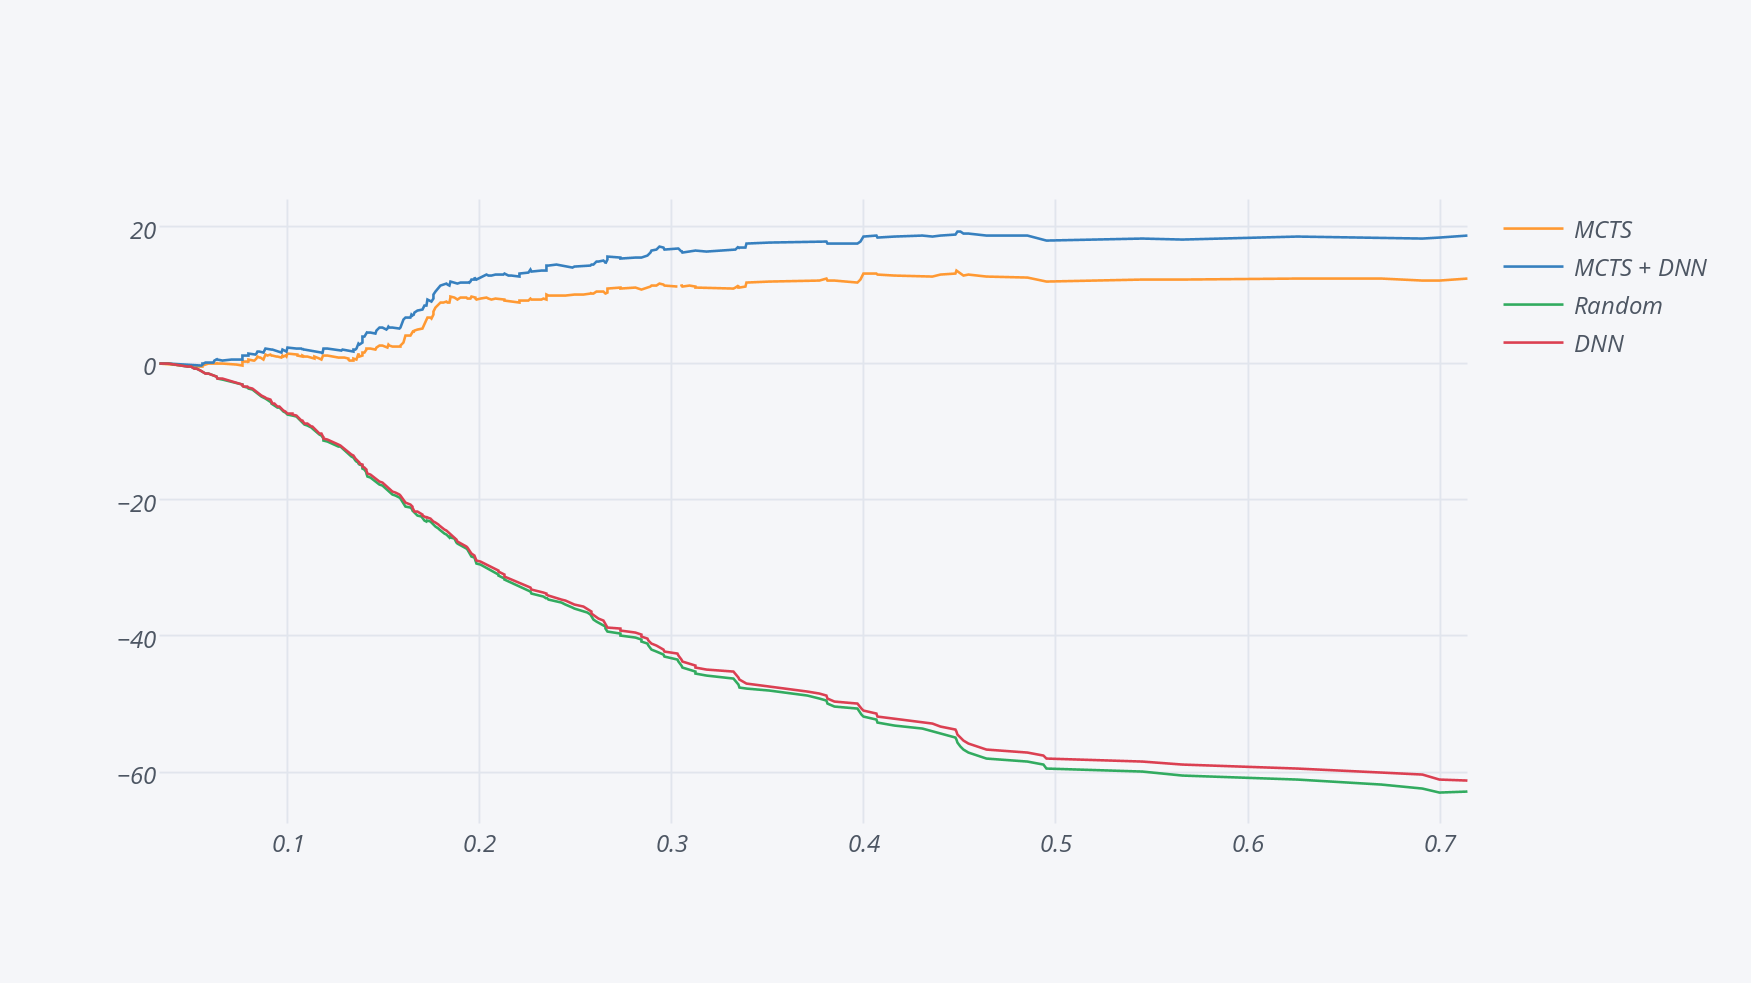
\includegraphics[width=\textwidth]{images/delta_sr.png}
\label{fig:delta_sr}
\caption{Delta success rate for each methods success rate}
\end{figure}

\begin{table}
\caption{Success rate for each method}
\centering
\begin{tabular}{l{c}r}
\hline\hline
Method & Mean & Standard deviation \\
\hline
MCTS + Random & 0.212663 & 0.226270 \\
MCTS + DNN & 0.229924 & 0.230549 \\
Random & 0.010199 & 0.066933 \\
DNN & 0.014281 & 0.046330 \\
\hline
\end{tabular}
\end{table}

\begin{table}
\caption{Statistical significances of improvements between methods}
\centering
\begin{tabular}{l{c}r}
\hline\hline
Residuals & Mean & P-value\\ 
\hline
(MCTS + DNN) - (MCTS + Random) & 0.0171 & 0.000366 \\
(DNN - Random) & 0.00408  & 0.0327238 \\
\hline
\end{tabular}
\end{table}
 
\chapter{Discussion}
\section{Training neural networks}
The validation accuracy on the simplified dataset is high and reaches 92.2\% as seen in Fig. \ref{fig:candy_small_validation_accuracy}. Given more data, more training time and a bigger model  it would likely be able to become even better. 

The validation accuracy on the Monte Carlo tree search data is much lower at around 27\% as seen in Fig. \ref{fig:candy_real_validation_accuracy}. This is not surprising as  it is generated from a non-deterministic algorithm. 27\% is still a lot higher than 16.3\% which random guessing would give. Given that we do not know how predictable the MCTS data is it is hard to know how good our network has been on learning it. It could be that 30\% is the theoretical maximum validation accuracy, in which case 27\% is good, or it could be much higher, in which case 27\% might be pretty bad. 

\section{Monte Carlo tree search}
Playing without any search, deep learning outperforms random and it improves MCTS when used during playouts as can be seen in Fig. \ref{fig:cumulative_sr}.  This demonstrates  that the neural network has learned useful knowledge of the game through from the data.  MCTS already outperformed average players, adding DNN makes it outperform average players even more, while DNN without any search underperforms average players as seen in Fig. \ref{fig:delta_sr}.  The neural network does not play  good enough on its own to be useful on its own. One of the problems with the training data is that it does not include goals of the game. For this reason alone its going to be difficult to perform well without any search.  It could also become stronger if it was trained on expert human moves instead of MCTS generated data. The improvement between using search or no search is much greater than the improvement between using deep learning or no deep learning. The gains from using deep learning must outweigh the fact that it takes quite a lot of work to train the neural network and that it will need to be continuously retrained when new features are added to the game in order for it to be worth continued usage in the future.

\section{Conclusions}
\begin{itemize}
\item Learning a heuristic from data works well
\item  Deep learning improves MCTS
\item  Deep learning without MCTS is not strong enough be useful on its own 
\end{itemize}

\chapter{Future work}
\section{Reinforcement learning}
In this thesis we only attempted to make the neural network learn how someone else plays  may it be real players or bots. The performance metric being minimized is how well the neural network can predict how someone else would play. It could be interesting to change the aim to play as good as possible. Using reinforcement learning the neural networks weights  could be altered after having been trained on a dataset to maximize its performance. Play a level, see how well it performed, update the weights in order to make it play better the next time. 

\section{Real user data}
We initially intended to use  real user data for this thesis. We spent a lot of time collecting  it for Candy Crush Soda Saga which required adding code to the code base and getting it released.  It was however aborted as there were problems replaying the games outside of our control.  It would be interesting to continue this experiment and train on expert players and see what that does for performance.

\section{Improve architecture}
As we were heavily restricted by time  we did not investigate the space of possible neural networks very much.  There is an almost infinite number of things one could try. If one has time then training a much deeper network with much more data would likely give better results.

\section{Use improved data}
The data we used excluded important information such as the goal of the level. Using better data would likely yield better results.

\section{Qualitative exploration of learning}
We only made quantitative measurements of performance. What kind of moves and strategies does the neural network learn? We have no idea, we only know that it gets a certain validation accuracy and that it gets a certain success rate in a game. Exploring what kind of moves  it learns and does not learn could perhaps give some interesting insights.

\bibliography{references}

\end{document}


